\section{Qualität}\label{sec:qualitat}
Die \textbf{Qualität} einer Software lässt sich oft nur schwer beschreiben.\\
Trotzdem ist es wichtig, sie genau zu definieren: Der Kunde möchte ein bestimmtes Maß an Mindestqualität vertraglich vereinbaren.
Als Entwickler muss man verstehen, was der Kunde unter Qualität versteht, um eine zufriedenstellende Arbeit abzuliefern.\\
Im Einsatz auf dem anonymen Markt stellt sich die Frage, wann die Qualität einer Software hoch genug ist, damit sie ausgeliefert werden kann.

\subsection*{Qualität ist entscheidend}
Die Qualität einer Software ist sicher entscheidend für ihren Erfolg: Wenn eine Software richtig funktioniert, ist sie zur Lösung bestimmter Probleme bzw. im Einsatz zur Erledigung bestimmter Aufgaben geeignet.\\
Hierzu muss sichergestellt sein, dass an entscheidenden (\textit{geschäftskritischen}) Stellen keine Probleme auftreten.\\
Außerdem muss die Software den Qualitätsforderungen (s. Abschnitt~\ref{sec:nicht-funktionale-anforderungen}) genügen.

\vspace{2mm}
\begin{tcolorbox}[title=Qualitätsforderung/Qualitätsanforderung]
    \textbf{Qualitätsforderungen} (auch: \textit{Qualitätsmerkmale}) helfen dabei, Qualitätsanforderungen zu konkretisieren (vgl.~\cite[58]{Wed09}).
\end{tcolorbox}

\subsection*{Qualitätssicherung}
Die Aufgabe der \textbf{Qualitätssicherung} liegt u.a. darin, sicherzustellen, dass die \textbf{Qualitätsforderungen} eingehalten werden.

\vspace{2mm}
\begin{tcolorbox}
    Für jede \textbf{Qualitätsforderung} muss mindestens eine \textbf{Maßnahme}\footnote{man spricht in diesem Zusammenhang von \textit{Qualitätsmaßnahmen}} vorhanden sein, die die Erfüllung dieser Qualitätsforderung gewährleistet (vgl.~\cite[1]{Wed09c})
\end{tcolorbox}
\vspace{2mm}

\noindent
Da eine möglichst kostengünstige Produktion von Software ein wesentliches Ziel des Software Engineering ist\footnote{
s. Teil 1, bspw. Abschnitt~\ref{sec:einfuhrung}
} und jede Maßnahme Geld kostet, muss sichergestellt werden, dass nur die \textit{absolut notwendigen} Qualitätsforderungen berücksichtigt werden und effiziente und effektive Qualitätsmaßnahmen ergriffen werden.

\subsection*{Qualitätssystem}
Aufgrund der unterschiedlichen Vorstellungen von \textbf{Qualitätsforderungen} werden diese genau definiert.\\
Hierzu wurden unterschiedliche \textbf{Qualitätssysteme} entwickelt, wie bspw. der Standard \textbf{IEEE 1061-1998}\footnote{s. Abschnitt~\ref{sec:nicht-funktionale-anforderungen}} oder \textbf{ISO 9126} als Grundlage für \textbf{ISO/IEC 25000:2005}\footnote{
    \url{https://www.iso.org/standard/35683.html}, abgerufen 20.05.2024
}.

\subsection*{Beispiel für Qualitätsforderung}
Ein Kunde fordert
\begin{itemize}
    \item eine hohe Effizienz einer Software
    \item insb. eine hohe Performance bei einem vorgegebenen Server, auf dem die Software laufen soll
\end{itemize}

\noindent
In weiteren Gesprächen stellt sich heraus, dass er darunter folgendes versteht:

\begin{itemize}
    \item eine geringe Antwortzeit des Systems im Onlinebetrieb
    \item einen hohen Datendurchsatz beim Massendatenimport
    \item Antwortzeiten, die nicht mehr als 1 Sekunde benötigen, und zwar
        \begin{itemize}
            \item unter Vollast des Systems
            \item bei 100 angemeldeten und gleichzeitig arbeitenden Benutzern
        \end{itemize}
    \item Verarbeitung von 50 Datensätze pro Minute bei einem Massenimport
\end{itemize}

\noindent
Es stellt sich heraus:

\begin{itemize}
    \item Der Begriff \textit{Effizienz} wird definiert durch
    \begin{itemize}
        \item den Begriff \textit{Performance}
        \item die Vorschrift einer \textit{Ressource} (\textbf{Verbrauchsverhalten})
    \end{itemize}
    \item \textbf{Performance} wird durch Forderungen nach \textit{Antwortzeit} und \textit{Datendurchsatz} konkretisiert
\end{itemize}

\noindent
Diese schrittweise Konkretisierung ist typisch.

\subsection*{Systematik von Qualitätssystemen}
Aufgrund der typischen schrittweisen Konkretisierung von Qualitätsforderungen sind Qualitätssysteme  \textit{hierarchisch} aufgebaut (s. Abbildung~\ref{fig:qualitätssysteme}):

\begin{itemize}
    \item \textbf{Qualität} wird definiert durch
    \begin{itemize}
        \item  \textbf{Qualitätsmerkmale} (bspw. ``\textit{Effizienz}``), die konkretisiert werden durch
        \begin{itemize}
            \item  \textbf{Qualitätsteilmerkmale} (bspw. ``\textit{Performance}``, ``\textit{Verbrauchsverhalten}``), die genau definiert werden durch
             \begin{itemize}
                       \item \textbf{Qualitätsindikatoren}, die jeweils einem \textit{Artefakt} innewohnende Eigenschaften beschreiben, die objektiv bestimmt werden kann (bspw. ``\textit{Antwortzeit}``, ``\textit{Datendurchsatz}``)
            \end{itemize}
        \end{itemize}
    \end{itemize}
\end{itemize}

\noindent
Zur Bestimmung von Qualitätsindikatoren werden \texbf{Metriken} eingesetzt, also ``\textit{Vorschriften}, anhand derer Zahlen berechnet werden können, die ein Maß für die Güte einer Software darstellen`` (\cite[3, Hervorhebung eigene]{Wed09c}).


\begin{figure}
    \centering
    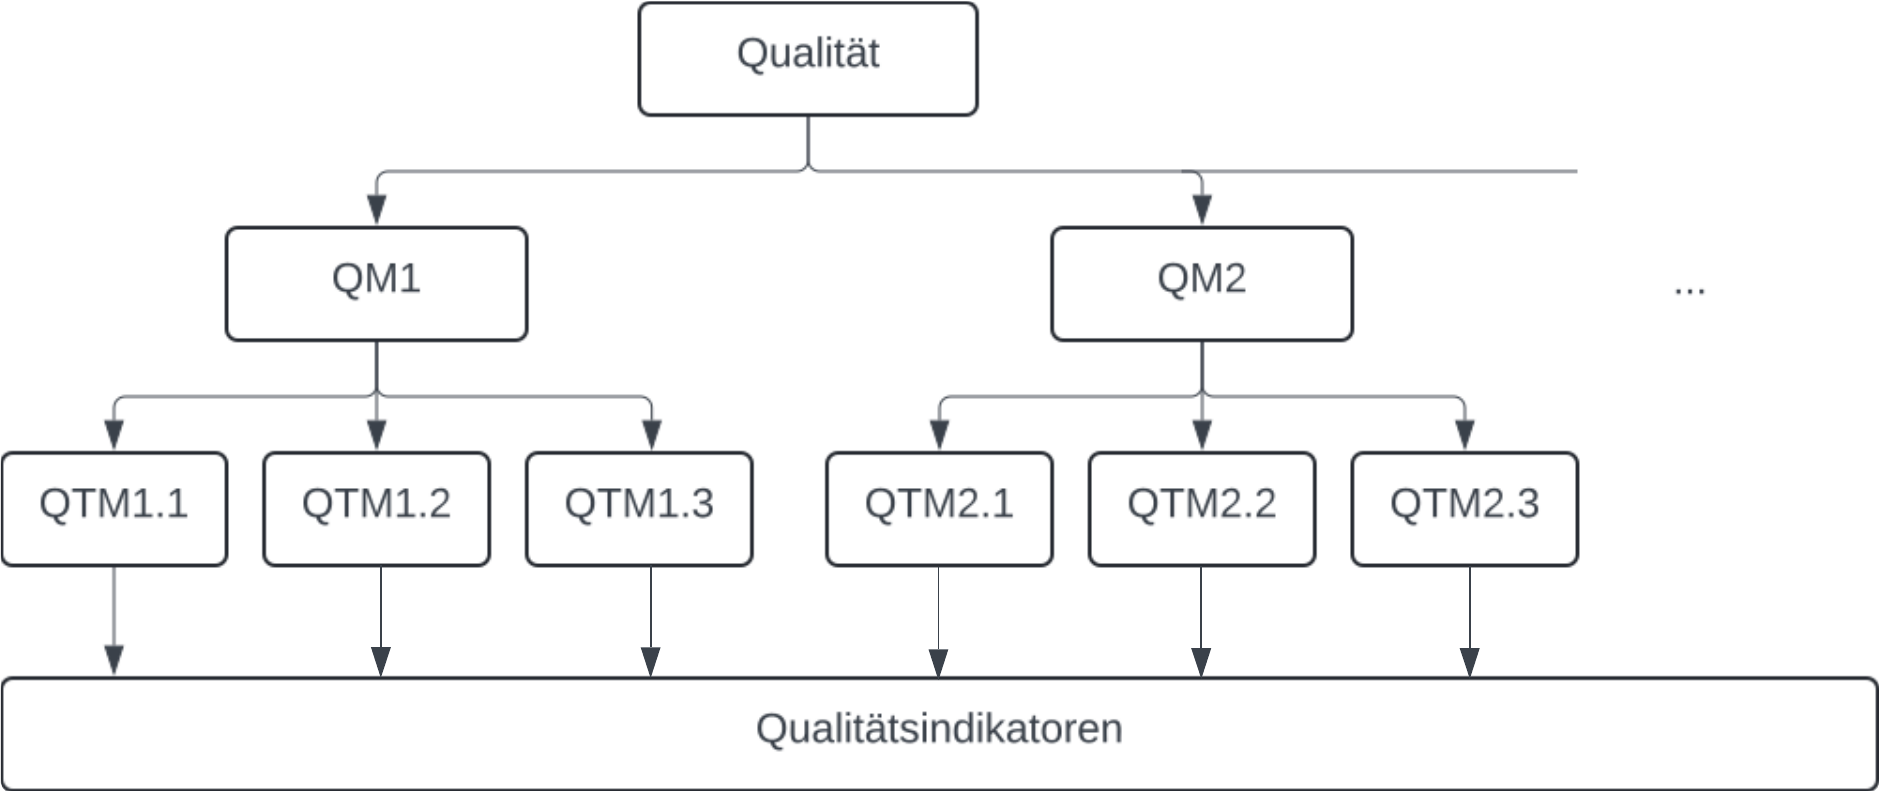
\includegraphics[scale=0.8]{part four/Qualität/img/qualitätssysteme}
    \caption{Skizzenhafter Aufbau von Qualitätssystemen. \textit{Qualitätsindikatoren} sind als breiter Balken dargestellt, da sich mehrere \textit{Qualitätsteilmerkmale} auf einen gemeinsamen \textit{Qualitätsindikator} beziehen können. (Quelle: in Anlehnung an~\cite[Abb. 1.1, 3]{Wed09c})}
    \label{fig:qualitätssysteme}
\end{figure}


\subsection*{Vorgehen}
Vorgegebene \textbf{Qualitätsmodelle} dienen als Vorlage für eine mögliche Definition von Begriffen (s. Abbildung~\ref{fig:qualitätsmerkmale}).\\
Dies ermöglicht die Auswahl von Qualitäts(teil)merkmalen, die für ein konkretes Projekt notwendig sind.\\
Es ist auch möglich, die passenden Merkmale selbst zu definieren.\\

\noindent
Des Weiteren existieren mögliche \textit{Messvorschriften} für \textbf{Qualitätsindikatoren} in den Standards.

\vspace{2mm}
\begin{tcolorbox}
    Damit definierte Qualitätsforderungen auch tatsächlich erreicht werden, müssen Maßnahmen geplant werden, die dies sicherstellen.\\
    Die Erfahrung zeigt, dass Qualitätsforderungen, die nicht überprüft werden, in der Regel auch nicht erfüllt werden (vgl.\cite[4]{Wed09c}).
\end{tcolorbox}
\vspace{2mm}


\begin{figure}
    \centering
    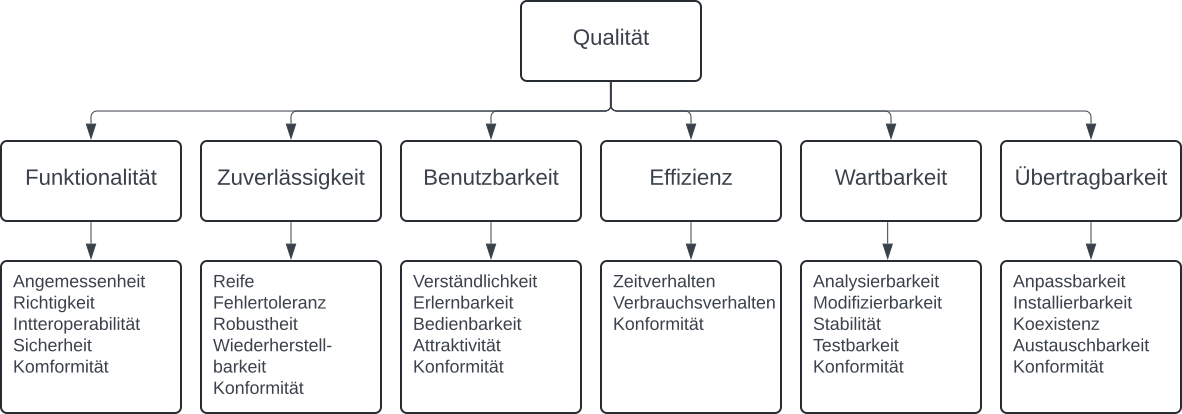
\includegraphics[scale=0.4]{part four/Qualität/img/qualitätsmerkmale}
    \caption{\textit{Qualitätsmerkmale} und -\textit{teilmerkmale} nach \textbf{ISO 9216}. (Quelle: in Anlehnung an~\cite[Abb. 1.2, 3]{Wed09c})}
    \label{fig:qualitätsmerkmale}
\end{figure}


\subsection*{Genaue Definition durch Szenarien}
Bleiben Qualitätsindikatoren zu abstrakt, ist für die Qualitätssicherung häufig unklar, was genau zu überprüfen ist.\\
Aus diesem Grund werden Qualitätsforderungen mittels \textbf{Szenarien} exakter beschrieben und für die Praxis damit nutzbar.\\
Ein \textbf{Qualitäts-Szenario} besteht aus folgenden Teilen (s. Abbildung:~\ref{fig:qualitätsszenario}):

\begin{enumerate}
    \item \textbf{Quelle des Stimulus}: \textit{Akteur} (Mensch, Computersystem, Hardware)
    \item \textbf{Stimulus}: \textit{Vorgang}, der etwas im System auslöst
    \item \textbf{Umgebung}: Der \textbf{Stimulus} tritt in einer Umgebung auf (bspw. ``System, mit dem 100 Benutzer gleichzeitig arbeiten``)
    \item \textbf{Artefakt}: Das gesamte System oder Teile davon (die \textit{Dokumentation} gehört auch dazu)
    \item \textbf{Antwort}: Die \textit{Aktivität}, die auf den \textbf{Stimulus} hin erwartet wird
    \item \textbf{Messvorschrift}: eine genau definierte \textit{Messung}, also so, dass sie \textit{objektiv messbar} ist
\end{enumerate}


\begin{figure}
    \centering
    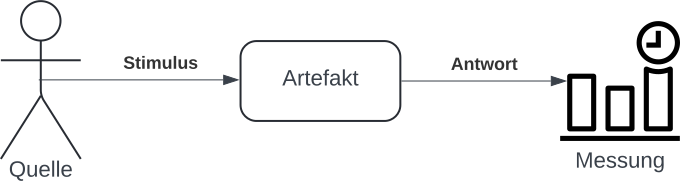
\includegraphics[scale=0.4]{part four/Qualität/img/qualitätsszenario}
    \caption{Skizze eine \textit{Qualitätsszenarios}. Eine \textbf{Umgebung}, in der der Stimulus auftritt, wird implizit vorausgesetzt. (Quelle: in Anlehnung an~\cite[Abb. 1.2, 4]{Wed09c})}
    \label{fig:qualitätsszenario}
\end{figure}


\noindent
Ein Qualitäts-Szenario für das o.a. Beispiel sieht demnach wie folgt aus:

\begin{enumerate}
    \item \textbf{Quelle des Stimulus}: Anwender
    \item \textbf{Stimulus}: Anwender löst in einem Dialog eine Aktion aus
    \item \textbf{Umgebung}: System, mit dem 100 Benutzer gleichzeitig arbeiten. Datenbank ist mit Daten gefüllt.
    \item \textbf{Artefakt}: Das System
    \item \textbf{Antwort}: Bestätigungsanzeige
    \item \textbf{Messvorschrift}: Zeit zwischen Auslösung der Aktion und Anzeige der Bestätigung. Muss gewartet werden, um weiterarbeiten zu können, ist die Zeit hinzuzuzählen. Wird das Legacy-System bei der Funktionalität genutzt, ist die Antwortzeit des Legacy-Systems getrennt zu messen und von der gesamten Antwortzeit abzuziehen.
\end{enumerate}

\subsection*{Priorisierung}
Unterschiedliche Qualitätsforderungen können sich manchmal in der Praxis widersprechen. Ein \textit{autocomplete}-Feld soll bspw. für die Benutzerfreundlichkeit implementiert werden, was aber zu Lasten eines niedrigen Verbrauchsverhaltens und niedriger Antwortzeiten führen kann.\\
Es muss also zwischen den verschiedenen Qualitätsforderungen abgewogen werden, da unterschiedliche Qualitätsforderungen auch unterschiedliche Auswirkungen auf den Erfolg haben können.\\
Deshalb sollten Qualitätsforderungen \textbf{priorisiert} werden

\subsection*{Notwendig, aber nicht hinreichend für den Erfolg}
Unter Berücksichtigung der aufgeführten Punkte können alle Beteiligte hinsichtlich der Qualitätsforderungen ein gemeinsames Verständnis erlangen.

\begin{tcolorbox}[title=Formale Qualitätsforderungen als Hilfsmittel]
    Qualitätsforderungen definieren für die Qualitätssicherung klare Aufgaben.\\
    Allerdings liegt Qualität nicht alleine dann vor, wenn Qualitätsforderungen erfüllt sind, sondern dann, wenn Kunden ein Produkt erhalten, das ihren Bedürfnissen entspricht.\\
    Formale Qualitätsforderungen sind ein \textbf{Hilfsmittel}, bieten aber keine Garantie  (vgl.~\cite[6]{Wed09c}).
\end{tcolorbox}